\clearpage
\section{Network architectures to represent CNF formulae}

In this section,  we design three architectures for the boolean function synthesis problem. Each of these architectures are used to learn formulae in conjunctive normal form (CNF).  The training phase is guided using an oracle that provides counterexamples to the formulae synthesized using the network.  In our setting, the oracle is a verifier for the boolean function synthesis problem.  In this problem,  for a given function, there could be multiple solutions possible and hence multiple local minima.  The choice of minima depends on the counterexamples generated by the counterexample loop.

\subsection{Architecture 1: Single output GCLN}

Let the CNF formula be $F$ as shown below:

\[ F = \bigwedge_{j = 1}^m \ (\  \bigvee_{i=1}^{2n}\  (x_i\ .\ g_{ij})\ .\ g_j)\]

where,  \\ 
$n$ = number of input variables (i.e.,  $|V_{in}|$), \\
$m$ = number of clauses and is bounded by $2^{2n}$ \\
$x_i$ = set of variables and their negations (i.e.,  $2|V_{in}|$), .\\
$g_{ij}$ = 1 iff the $i^{th}$ variable is used in the $j^{th}$ clause.\\
$g_{j}$ = 1 iff the $j^{th}$ clause is used for the output.\\

The GCLN architecture for $m = 3$ and $V_{in} = \{ x\}$ is as \ref{fig:arch1}. \\

\begin{figure}[t]
	\centering
    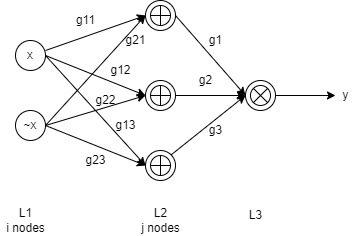
\includegraphics[scale=0.5]{architecture-1.png}
    \caption{Architecture 1: Single Output GCLN}
    \label{fig:arch1}
\end{figure}

The network has three layers where the middle (disjunct) layer is variable in size.

Although this network has a single output,  we may be able to synthesize functions for multiple outputs by:\\
(a) sampling intelligently,  \\
(b)using a dependency guided loop after every function synthesized (not sure how as we do not know how to extract a single correct function separately)

\subsection{Architecture 2: Multiple output GCLN with a shared layer}

In this setting, for each of the $l$ output variables in the boolean function synthesis problem, we wish to synthesize a formula $F_k$ such that:

\[ F_k = \bigwedge_{j = 1}^m \ (\  \bigvee_{i=1}^{2n}\  (x_i\ .\ g_{ij})\ .\ g_{jk}), \ \ \ k \in \{1, ..., l\}\]

where,  \\ 

$l$ = number of output variables (i.e.,  $|V_{out}|$), \\
$g_{jk}$ = 1 iff the $j^{th}$ clause is used for the $k^{th}$ output.\\
and the rest are as before.

The GCLN architecture for $m = 3$,  $V_{in} = \{ x\}$, and $V_{out} = \{ y_1, y_2\}$ is as \ref{fig:arch2}. \\

\begin{figure}[t]
	\centering
    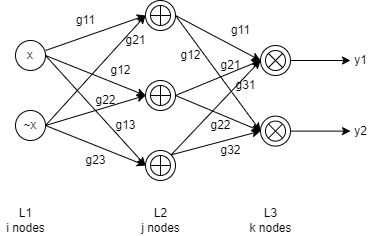
\includegraphics[scale=0.5]{architecture-2.png}
    \caption{Architecture 2: Multiple output GCLN with a shared layer}
    \label{fig:arch2}
\end{figure}

As observed,  the middle layer is shared between all the $l$ outputs.
\subsection{Architecture 3: Multiple output GCLN without a shared layer}

In this setting, we extend the above architecture and assign $m$ nodes to each of the $l$ outputs. Thus, we now have $ml$ nodes in the middle layer.

Thus, $F_k$ is now:
\[ F_k = \bigwedge_{j = mk-m-1}^{mk} \ (\  \bigvee_{i=1}^{2n}\  (x_i\ .\ g_{ij})\ .\ g_{jk}), \ \ \ k \in \{1, ..., l\}\]

where a block $B_k$ for an output $k$ ranges from $mk-m-1$ to $mk$, for a given output $k$, for $m$ clauses.

The GCLN architecture for $m = 3$,  $V_{in} = \{ x\}$, and $V_{out} = \{ y_1, y_2\}$ is as \ref{fig:arch3} \\

\begin{figure}[t]
	\centering
    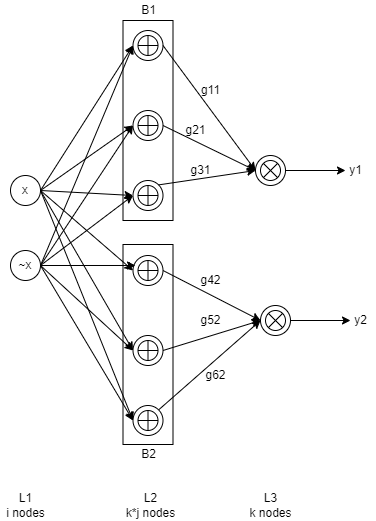
\includegraphics[scale=0.5]{architecture-3.png}
    \caption{Architecture 3: Multiple output GCLN without a shared layer}
    \label{fig:arch3}
\end{figure}

\section{Network architecture to represent DNF formulae}

The architectures used to synthesize CNF formulae can also be used to learn formulae in disjunctive normal form (DNF).  In such a case, the middle layer would now consist of T-conorms instead of T-norms.

\section{Possible advantages of our approach over Manthan}
\begin{itemize}
\item Manthan is constrained to use DNF formulae only whereas we can use both CNF and DNF as the size of the formula is within our reach.  $SAT \leq_P 3-SAT$ tells us that for any formula there exists an equisatisfiable formula in CNF of polynomial size.  No  such result is known for DNF.  All such reductions give an exponentially sized DNF formulae. Can we somehow expect, using this information, that we can generate smaller formulae?

\end{itemize}